%2multibyte Version: 5.50.0.2960 CodePage: 65001
\documentclass[letterpaper,12pt]{article}%
\usepackage{amssymb}
\usepackage{amsmath}
\usepackage{float}
\usepackage[toc,page]{appendix}
\usepackage[doublespacing]{setspace}
\usepackage{geometry}
\usepackage{amsfonts}
\usepackage{tabularx}
\usepackage{array}
\usepackage{graphicx}
\usepackage{booktabs}
\usepackage{threeparttable}

\usepackage[format=default,labelsep=newline,justification=centering,width=0.95\textwidth
]{caption}


\geometry{left=0.75in,right=0.75in,top=0.75in,bottom=0.75in}
\begin{document}

\title{ECON 722 Term Paper: Monetary and fiscal policy interactions}
\author{Yoshiki Ando and Joao Ritto}
\maketitle
% Let me call Leeper et al. (2017) by LTW

\section{Introduction}

In this term paper we wanted to work with the model developed in Leeper et al. (2017) (LTW, henceforth) for a variety of reasons. Firstly, the topic of the effects of Fiscal Policy seemed to us interesting and far from settled, hence studying this model could help us get better acquainted with the literature and how to potentially tackle questions about fiscal multipliers under different settings. Secondly, the fact that the model is reasonably large made our task challenging in a good way, allowing us to to take a develop our DSGE estimation skills more thoroughly. Thirdly, we thought about specific things that would be interesting to do with this model, once we had replicated the paper's work.

The last of these reasons proved to be part of an overly ambitious and somewhat optimistic plan. Unfortunately, the replicating process proved itself a lot more cumbersome than we had expected, leaving us no time to go further. However, a brighter reading of this is that we ended up learning a lot more than we initially thought was needed for the replication of the paper.

As will be seen below, we coded the model in Julia and replicated some of its main tables. Computing time also caught us unprepared: LTW run the Random Walk Metropolis Hastings algorithm with 1.5 million draws, but we ended up not doing it with more than 100 thousand. Even this number took more than 24 hours in our laptops and we had trouble finding obvious ways of making our code more efficient.

In the section that follows we discuss our implementation. Section 3 presents the main results we replicated, discussing how they differ from the paper's. The last section concludes.

\section{Implementation}

Our code is publicly available on github: https://github.com/joaoritto/722TermPaper.git

\subsection{Prior Predictive Analysis}

LTW starts with a Prior Predictive Analysis in which different versions of the model are simulating, taking parameter draws from a prior distribution to study the range of fiscal multipliers that each of these submodels can generate. We replicated these results with N=20,000 as LTW. Our results are very similar but not exactly similar to the second decimal.

\subsubsection*{Prior Distribution}
We follow Table 2 in LTW for prior distributions. There are 34 parameters. The prior distributions include Normal, Gamma, Beta, Uniform, and Inverse Gamma distribution. The parameters  governing the distribution (e.g. shape and scale parameters in the Gamma distribution) are set to yield a particular mean and standard deviation. Therefore, the first task is converting the mean ($\mu$) and standard deviation ($\sigma$) to the shape/scale parameters in each distribution. For example, $\alpha$ (shape) and $\beta$ (scale) parameters in Gamma distribution is set to be:
\begin{align*}
\alpha = \left( \mu/\sigma  \right)^2, \ \beta = \sigma^2/\mu 
\end{align*}
Since $\xi$ follows the Gamma distribution with $\mu=2, \ \sigma=0.5$, we draw $\xi$ from $Gamma(\alpha=16, \beta=8)$. To evaluate the density for a specific value of $\xi$, we apply the density function to the value $x$:
\begin{align*}
f(x; \alpha, \beta) = \frac{x^{\alpha-1}  e^{-x/\beta }}{\Gamma(\alpha) \beta^\alpha}
\end{align*}
Since the package ``Distribution.jl'' contains this density function, we can draw $\xi$ by the command $rand(Gamma(\alpha,\beta))$ and evaluate the density at $x$ by $pdf(Gamma(\alpha,\beta), x )$. The procedures are the same for other values. All the parameters are drawn by the function $DrawParaFromPrior( )$, and all the parameter densities are evaluated by the function $ParaDensity(paraValues )$, where $paraValues$ is the vector of parameters.


\subsubsection*{Solving the Model}
To solve the model we use the method developed by Chris Sims to solve Linear Rational Expectations Models. We use the log-linearized equations provided in the appendix of LTW and write the matrices to have our system of equations in the form $\Gamma_0 y_{t}=\Gamma_1 y_{t-1}+Const+\Psi z_t+\Pi \eta_t$ where $z_t$ are the innovations and $\eta_t$ are expectation errors. These matrices are then used to get a backward-looking solution to the model $y_t=\Theta y_{t-1}+ \Phi z_t$, which we use as the transition equation for our model in state space form combined with an observables equation which is easy to define. 

For "gensys", the code that solves the model, we found an online version of it for Julia. This version, however, had been written for the version v 0.4 of Julia, which is not the most recent. Hence, we had to modify their code as a lot of the functions used had changed syntax in the more recent Julia versions.

We apply the different model restrictions by having a function which takes the model type and imposes the relevant restrictions before inputting the parameter vector into our function that solves the model.

\subsubsection*{Multipliers}
We follow LTW's description of the multipliers to compute these once we have drawed a parameter vector from the prior and solved the model.

\subsection{Bayesian Estimation of the Model}
We estimate the model using the Random Walk Metropolis Hastings. To do so, we initialize the procedure using the mean and inverse hessian mode that we took from LTW.

\subsubsection*{Data}
Following LTW, we use the US data from 1955:I to 2007:IV to focus in the pre-financial crisis periods. The data is contained in the file ``data.mat'' from their replication folder. There are 8 variables: $[C, I, w, GC, B, L, Pi, R]$ (log differences of aggregate consumption, investment, real wages, real government consumption, the real market-value of government debt, log hours worked, the GDP deflator, and the federal funds rate).

\subsubsection*{Kalman Filter}
Running the Kalman filter and evaluating the likelihood of the parameters given the data is standard. We follow the following notation:
\begin{align*}
\alpha_t &= T \alpha_{t-1} + R \eta_t, \ \text{where } \eta_t \sim N(0,Q) \\
y_t &= Z \alpha_t + \epsilon_t + W, \ \text{where } \epsilon_t \sim N(0,H)
\end{align*}
Then, the Kalman filter is computed in the recursive way:
\begin{align*}
a_{t/t-1} &= T a_{t-1} \\
P_{t/t-1} &= T P_{t-1} T' + R Q R' \\
a_t &= a_{t/t-1} + P_{t/t-1} Z' F_t^{-1} v_t\\
P_t &= P_{t/t-1} - P_{t/t-1} Z' F_t^{-1} Z P_{t/t-1} \\
\text{where } F_t&= Z P_{t/t-1} Z' + H, \ v_t = y_t - Z a_{t/t-1} - W,
\end{align*}
with the proper initialization. Finally, the likelihood is given by:
\begin{align*}
\ln L = -\frac{NT}{2} \ln 2\pi - \frac{1}{2} \sum_{t=1}^{T} \ln |F_t| - \frac{1}{2} \sum_{t=1}^T v_t' F_t^{-1} v_t,
\end{align*}
where $N,T$ denote the dimension of observables and the number of periods.

\subsubsection*{Random Walk Metropolis Hastings}
As LTW, we use the Random Walk Metropolis Hastings. We initialize it using their mode and inverse hessian mode. As part of the initialization we start with a step of c=1 to get the initial draw, after this we use c=0.28 in the main part of the algorithm (these values are the same ones used by LTW). We run only 100,000 draws, instead of 1,500,000 due to computational constraints and for the moments we present in our tables we discard the first 5000 draws.

\section{Results}
The first 3 tables we present show our results for the prior predictive analysis. They attempt to replicate tables 3 and 4 of LTW. The numbers tell us, for each of the model versions, what is the prior probability that the fiscal multipliers on output, consumption or investment are large, for different time horizons. Some of our numbers do not match LTW to the second decimal, but they are quite close. We use stars in our tables to denote how our results compare to LTW, as is easily seen we our replication is quite close to theirs, with the exception of model 4, regime M, complements with no taxes. It was unclear to us which restrictions are different in their work relative to the ones we imposed that could explain those divergences.

Below the tables we replicate figures 1 and 2.


\begin{table}[H]
    \centering
    \begin{threeparttable}
    \caption{Government Spending Output Multiplier Probabilities Implied By Prior Predictive Analysis Based on 20,000 Draws From the Prior Distribution}
    \begin{tabular}{l c c c c c}
    \toprule
        & \multicolumn{5}{c}{$Pr\Big(PV \frac{\triangle Y}{\triangle G}>1\Big)$}\\
      \cmidrule{2-6}
        & Impact & 4 qtrs & 10 qrts & 25 qrts & 10 years \\
       \midrule
     Model 1: RBC real frictions & 0.00***   & 0.00***  & 0.00***  & 0.00***  & 0.00*** \\
     Model 2: New Keynesian sticky prices and wages  &    &   &   &   &       \\
     \quad Regime M & 0.12** & 0.01*** & 0.01** & 0.01** & 0.01***  \\
     \quad Regime F, short debt & 1.00*** &  0.98***  & 0.94*** & 0.92***  & 0.92***  \\
     \quad Regime F, long debt &  0.96*** & 0.75* & 0.68** &  0.68***  & 0.68***  \\
     Model 3: New Keynesian non-savers &    &   &   &   &  \\
     \quad Regime M &   0.58*** & 0.16 & 0.06***  & 0.04*** & 0.04** \\
     \quad Regime F, short debt &  1.00*** &  0.99**  & 0.96** & 0.95***  & 0.94*** \\
     \quad Regime F, long debt &   1.00*** & 0.91* & 0.80** & 0.77***  & 0.76*** \\
     Model 4: New Keynesian G in utility &    &   &   &   &  \\
     \quad Regime M, substitutes &   0.01** & 0.00*** & 0.00***  & 0.01**  & 0.01**  \\
     \quad Regime M, complements &   0.84*** &  0.64* &  0.47**  & 0.33***  & 0.29***  \\
     \quad Regime M, complements, ss tax only &   0.84** & 0.63*  & 0.48** & 0.41** & 0.40**  \\
     \quad Regime M, complements, no tax &   0.73 &  0.40 & 0.23  & 0.18 & 0.17 \\
     \quad Regime F, substitutes, short debt &  0.43*** & 0.51*  & 0.68*  & 0.79** & 0.81**  \\
     \quad Regime F, substitutes, long debt &  0.22**  & 0.17**  & 0.23** &  0.39**  & 0.45** \\
     \quad Regime F, complements, short debt &   1.00*** & 1.00*** & 0.99*** & 0.97*** & 0.97***  \\
     \quad Regime F, complements, long debt &  1.00*** & 0.97**  & 0.92** &  0.88*** & 0.86***  \\
     \quad Regime F, complements, short debt, ss tax only &  1.00***   &   1.00*** & 0.99*** & 0.97*** & 0.97***  \\
     \quad Regime F, complements, long debt, ss tax only &  1.00*** & 0.97** &  0.92** &  0.88*** & 0.86***\\
     \quad Regime F, complements, short debt, no tax &  1.00*** & 1.00*** &  0.99*** & 0.99***  & 0.98*** \\
     \quad Regime F, complements, long debt, no tax &   1.00*** &  0.98**  & 0.95***  & 0.92*** & 0.91***  \\
     \midrule
    \bottomrule    
    \end{tabular}
    \begin{tablenotes}
    \item * stands for a difference below 0.05 relative to LTW, ** stands for a difference below 0.02, *** stands for a correct value to the second decimal
    \end{tablenotes}
    \label{tab:PPAOutputMultipliers}
    \end{threeparttable}
\end{table}

\begin{table}[H]
    \centering
    \begin{threeparttable}
     \caption{Government Spending Consumption Multiplier Probabilities Implied By Prior Predictive Analysis Based on 20,000 Draws From the Prior Distribution}
    \begin{tabular}{l c c c c c}
    \toprule
        & \multicolumn{5}{c}{$Pr\Big(PV \frac{\triangle C}{\triangle G}>0\Big)$}\\
        \cmidrule{2-6}
        & Impact & 4 qtrs & 10 qrts & 25 qrts & 10 years \\
        \midrule
     Model 1: RBC real frictions &  0.00***   & 0.00***  & 0.00***  & 0.00***  & 0.00*** \\
     Model 2: New Keynesian sticky prices and wages    &    &   &   &   &  \\
     \quad Regime M &   0.01** &  0.00***  & 0.00*** & 0.01** & 0.01***  \\
     \quad Regime F, short debt &  0.98*** & 0.95** &  0.91**  & 0.90***  & 0.89***  \\
     \quad Regime F, long debt &  0.78**  &  0.53* & 0.50** & 0.55*** & 0.57**  \\
     Model 3: New Keynesian non-savers &    &   &   &   &  \\
     \quad Regime M &  0.49** &  0.16* & 0.08** & 0.05*** & 0.04*** \\
     \quad Regime F, short debt &  1.00*** & 0.99***  & 0.97** &  0.95** &  0.94** \\
     \quad Regime F, long debt &  0.99*** &  0.89*  & 0.81** & 0.76**  & 0.73**  \\
     Model 4: New Keynesian G in utility &    &   &   &   &  \\
     \quad Regime M, substitutes &  0.00*** &  0.00*** & 0.00*** & 0.00*** & 0.00***  \\
     \quad Regime M, complements &   0.82**  & 0.73**  & 0.69** & 0.60**  & 0.50** \\
     \quad Regime M, complements, ss tax only & 0.82*** & 0.71* &  0.67* & 0.60* & 0.55*  \\
     \quad Regime M, complements, no tax &  0.76  & 0.57  & 0.46 & 0.30  & 0.24  \\
     \quad Regime F, substitutes, short debt & 0.31** & 0.27***  & 0.30**  & 0.50** & 0.60**  \\
     \quad Regime F, substitutes, long debt &   0.12** & 0.06**  & 0.06*** & 0.13***  & 0.20**  \\
     \quad Regime F, complements, short debt &  1.00*** &  1.00*** & 0.99***  & 0.99*** & 0.98***  \\
     \quad Regime F, complements, long debt &  0.99*** & 0.96**  & 0.94*** & 0.92***  &  0.90*** \\
     \quad Regime F, complements, short debt, ss tax only &  1.00*** &  1.00*** &  0.99*** & 0.99*** & 0.98*** \\
     \quad Regime F, complements, long debt, ss tax only &  0.99***  & 0.96** & 0.94*** & 0.92**  & 0.90*** \\
     \quad Regime F, complements, short debt, no tax &  1.00*** & 1.00*** &  1.00*** & 0.99*** & 0.99*** \\
     \quad Regime F, complements, long debt, no tax &    1.00***  & 0.98***  & 0.97*** & 0.95** & 0.94*** \\
    \bottomrule    
    \end{tabular}
    \begin{tablenotes}
    \item * stands for a difference below 0.05 relative to LTW, ** stands for a difference below 0.02, *** stands for a correct value to the second decimal
    \end{tablenotes}
    \label{tab:my_label}
    \end{threeparttable}
\end{table}


\begin{table}[H]
    \centering
    \begin{threeparttable}
    \caption{Government Spending Investment Multiplier Probabilities Implied By Prior Predictive Analysis Based on 20,000 Draws From the Prior Distribution}
    \begin{tabular}{l c c c c c}
    \toprule
        & \multicolumn{5}{c}{$Pr\Big(PV \frac{\triangle I}{\triangle G}>0\Big)$}\\
        \cmidrule{2-6}
        & Impact & 4 qtrs & 10 qrts & 25 qrts & 10 years \\
        \midrule
     Model 1: RBC real frictions &  0.00***   & 0.00***  & 0.00***  & 0.00***  & 0.00***  \\
     Model 2: New Keynesian sticky prices and wages   &    &   &   &   &   \\
     \quad Regime M &  0.01** &  0.01** & 0.01**  & 0.01** &  0.01** \\
     \quad Regime F, short debt &   0.96*** &  0.87** & 0.82*** & 0.81*** & 0.81*** \\
     \quad Regime F, long debt &  0.63** & 0.50*** & 0.50*** & 0.56** & 0.57***  \\
     Model 3: New Keynesian non-savers &    &   &   &   &  \\
     \quad Regime M &  0.01** &  0.01** & 0.01** & 0.01**  & 0.01*** \\
     \quad Regime F, short debt &  0.91*** & 0.78* & 0.73** & 0.73** & 0.73**  \\
     \quad Regime F, long debt &   0.43***  &  0.31** & 0.35** & 0.43***  & 0.45** \\
     Model 4: New Keynesian G in utility &    &   &   &   &  \\
     \quad Regime M, substitutes &   0.36** & 0.30** & 0.19** & 0.07*** & 0.05**  \\
     \quad Regime M, complements &   0.01**  & 0.00***  & 0.01**  & 0.01**  & 0.01***  \\
     \quad Regime M, complements, ss tax only &  0.05* &  0.04*  & 0.04* & 0.04*  & 0.05*  \\
     \quad Regime M, complements, no tax &   0.03* & 0.02** &  0.02**  & 0.02**  & 0.02*** \\
     \quad Regime F, substitutes, short debt &   0.99** &  0.98*** & 0.96***  & 0.96***  & 0.96*** \\
     \quad Regime F, substitutes, long debt &   0.94*** &  0.90** &  0.89*** & 0.89*** & 0.90** \\
     \quad Regime F, complements, short debt &  0.67*** & 0.54**  &  0.54** & 0.59** & 0.60**  \\
     \quad Regime F, complements, long debt &   0.19*** & 0.12** & 0.14*** & 0.22***  & 0.25** \\
     \quad Regime F, complements, short debt, ss tax only &  0.67*** & 0.53** & 0.54**  & 0.58*** & 0.59*** \\
     \quad Regime F, complements, long debt, ss tax only &  0.20**  & 0.13*** & 0.15**  & 0.23**  &  0.26*** \\
     \quad Regime F, complements, short debt, no tax &  0.92*** & 0.81**   & 0.76***  & 0.75***  & 0.75*** \\
     \quad Regime F, complements, long debt, no tax &   0.43*** & 0.35*** & 0.37**  & 0.43*** & 0.45** \\
    \bottomrule    
    \end{tabular}
    \begin{tablenotes}
    \item * stands for a difference below 0.05 relative to LTW, ** stands for a difference below 0.02, *** stands for a correct value to the second decimal
    \end{tablenotes}
    \label{tab:my_label}
    \end{threeparttable}
\end{table}

\begin{figure}[H]
    \centering
    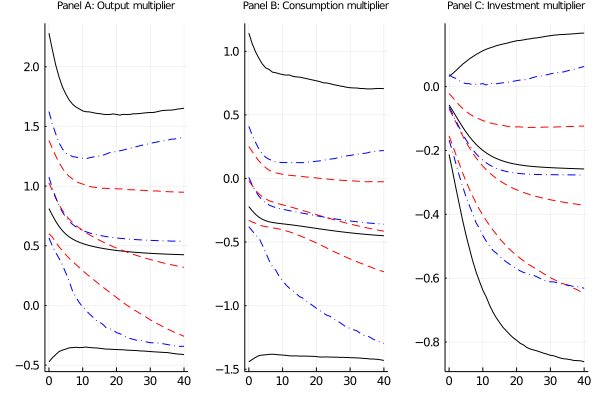
\includegraphics[width=12cm]{figure1.png}
    \caption{Present value multipliers in regime M with 90 percent confidence bands: Government spending in utility unrestricted, steady-state taxes
only, long debt (solid lines); rule-of-thumb agents, everything responds to debt, long debt (dashed lines); rule-ofthumb
agents, steady-state taxes only, long debt (dotted-dashed lines) }
    \label{fig:my_label}
\end{figure}


\begin{figure}[H]
    \centering
    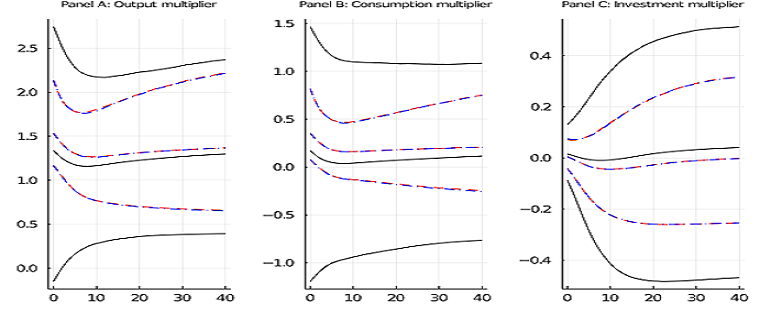
\includegraphics[width=12cm]{figure2.png}
    \caption{Present value multipliers in regime M with 90 percent confidence bands: Government spending in utility unrestricted, steady-state taxes
only, long debt (solid lines); rule-of-thumb agents, everything responds to debt, long debt (dashed lines); rule-ofthumb
agents, steady-state taxes only, long debt (dotted-dashed lines) }
    \label{fig:my_label}
\end{figure}

The tables that follow reproduce tables 5, 7 and 8 of LTW, presenting our results for the bayesian estimation of the model. Obviously our results here are a bit less close to LTW given the significantly larger number of draws that they did. Overall, we find our results to have the same type of messages and our IRFs, which we plot below the tables, look satisfactorily similar to theirs.

%% Counterpart of Table 5
\begin{table}[H]
	\centering
	\begin{threeparttable}
		\caption{Posterior Distribution for Estimated Parameters (Table 5 in LTW)}
		\begin{tabular}{l c c  c c}
			\toprule
			& \multicolumn{4}{c}{Our Results}  \\
			\cmidrule{2-5}
			Parameter & \multicolumn{2}{c}{Regime M} & \multicolumn{2}{c}{Regime F}\\
			& Mean & 90\% CS & Mean &  90\% CS \\
			\midrule
			Preferences and HHs&     &   &  &    \\
			\quad $\xi$, inverse Frisch labor elasticity&  1.70 & [1.11,2.42] & 2.35 & [1.59,3.22]  \\
			\quad $\theta$, habit formation & 1.00 & [0.99,1.0]& 0.99 & [0.98,0.99]\\
			\quad $\alpha_G$, G in utility & -0.23 & [-0.39,-0.06] & -0.20 & [-0.37,-0.03] \\
			Friction and production&     &   &  &    \\
			\quad $100\gamma$, ss tech growth&  0.30 & [0.24,0.37] & 0.32 & [0.25,0.39]  \\
			\quad $\psi$, capital utilization & 0.16 & [0.09,0.23]& 0.15 & [0.08,0.23] \\
			\quad $s$, inv adj cost & 5.50 & [3.91,7.44]& 4.63 & [3.16,6.23] \\
			\quad $\omega_p$, price stickiness&  0.93 & [0.91,0.94]& 0.95 & [0.94,0.96]  \\
			\quad $\omega_w$, price stickiness&  0.92 & [0.89,0.94]& 0.87 & [0.83,0.90]  \\
			\quad $\chi_p$, price indexation&  0.06 & [0.02,0.13] & 0.06 & [0.02,0.13] \\
			\quad $\chi_w$, wage indexation&  0.18 & [0.11,0.26] & 0.18 & [0.1,0.26]\\
			Monetary Policy&     &   &  &    \\
			\quad $\phi_\pi$, interest rate response to inflation&  0.93 & [0.79,1.08] & 0.15 & [0.08,0.24] \\
			\quad $\phi_y$, interest rate response to output & 0.09 & [0.07,0.11]& 0.14 & [0.11,0.16] \\
			\quad $\rho_r$, lagged interest rate response & 0.71 & [0.64,0.77] & 0.15 & [0.07,0.23] \\ 
			Fiscal Policy&     &   &  &    \\
			\quad $\gamma_G$, government cons. response to debt&  0.23 & [0.16,0.31]& 0.0001 & [-0.0015,0.0017]  \\
			\quad $\gamma_Z$, transfer response to debt & -0.10 & [-0.19,-0.02] & 0.0000 & [-0.0016,0.0017]\\
			\quad $\rho_G$, lagged govt cons. response & 0.98 & [0.98,0.99] & 0.99 & [0.99,0.99]\\
			\quad $\rho_Z$, lagged transfer response & NE&  & 0.98 & [0.96,0.99] \\
			& \multicolumn{4}{c}{LTW}  \\
			\cmidrule{2-5} 
			Preferences and HHs&     &   &  &    \\
			\quad $\xi$, inverse Frisch labor elasticity&  1.54 & [0.92,2.14] & 2.32 & [1.49,3.20]  \\
			\quad $\theta$, habit formation & 0.99& [0.98,1.00] & 0.99 & [0.98,1.00] \\
			\quad $\alpha_G$, G in utility & -0.19& [-0.36,-0.02] & -0.16 & [-0.34,-0.02] \\
			Friction and production&     &   &  &    \\
			\quad $100\gamma$, ss tech growth&  0.24 & [0.18,0.31] & 0.27 & [0.20,0.33]  \\
			\quad $\psi$, capital utilization & 0.13& [0.08,0.17] & 0.13 & [0.06,0.19] \\
			\quad $s$, inv adj cost & 5.21& [3.68,6.71] & 3.97 & [2.47,5.36] \\
			\quad $\omega_p$, price stickiness&  0.89 & [0.86,0.91] & 0.95& [0.94,0.96]  \\
			\quad $\omega_w$, price stickiness&  0.87 & [0.83,0.92] & 0.85& [0.81,0.89]  \\
			\quad $\chi_p$, price indexation&  0.06 & [0.01,0.11] & 0.06& [0.01,0.11]  \\
			\quad $\chi_w$, wage indexation&  0.09 & [0.03,0.15] & 0.09& [0.03,0.15]  \\
			Monetary Policy&     &   &  &    \\
			\quad $\phi_\pi$, interest rate response to inflation&  1.14 & [0.98,1.31] & 0.15 & [0.08,0.23]  \\
			\quad $\phi_y$, interest rate response to output & 0.18& [0.13,0.22] & 0.17 & [0.14,0.20] \\
			\quad $\rho_r$, lagged interest rate response & 0.76& [0.71,0.81] & 0.15 & [0.06,0.23] \\ 
			Fiscal Policy&     &   &  &    \\
			\quad $\gamma_G$, government cons. response to debt&  0.21 & [0.13,0.30] & 0.0000 & [-0.0017,0.0016]  \\
			\quad $\gamma_G$, transfer response to debt & -0.03& [-0.13,0.08] & 0.0000& [-0.0017,0.0016] \\
			\quad $\rho_G$, lagged govt cons. response & 0.98& [0.98,0.99] & 0.98& [0.98,0.99] \\
			\quad $\rho_Z$, lagged transfer response & NE&  & 0.98 & [0.97,0.99] \\
						\bottomrule   
		\end{tabular}
		\begin{tablenotes}
			\item % Table shows means and 90 percent credible sets (CS). NE denotes not estimated.
		\end{tablenotes}
		\label{tab:RWMH_para}
	\end{threeparttable}
\end{table}

%% Counterpart of Table 7
\begin{table}[H]
	\centering
	\begin{threeparttable}
		\caption{Multipliers for Regime M (Table 7 in LTW)}
		\begin{tabular}{l c c c c c}
			\toprule
			& \multicolumn{5}{c}{$PV \frac{\triangle X}{\triangle G} , \ X \in \{Y,C,I\}$}\\
			\cmidrule{2-6}
			& Impact & 4 qtrs & 10 qrts & 25 qrts & 10 years \\
			\midrule
		    Our Results&     &   &  &   &   \\
			\quad Output Multiplier ($PV \frac{ \triangle Y}{\triangle G}$)&  1.35 & 1.1 & 0.86 & 0.67 & 0.68 \\
			\quad &   [1.16,1.53] & [0.92,1.28] & [0.68,1.05] & [0.46,0.9] & [0.44,0.94] \\
			\quad Consumption Multiplier ($PV \frac{ \triangle C}{\triangle G}$)&  0.23 & 0.22 & 0.22 & 0.21 & 0.22\\
			\quad &   [0.06,0.39] & [0.06,0.38] & [0.05,0.38] & [0.05,0.37] & [0.04,0.39] \\
			\quad Investment Multiplier ($PV \frac{ \triangle I}{\triangle G}$)&  -0.14 & -0.35 & -0.59 & -0.92 & -1.13 \\
			\quad &   [-0.19,-0.1] & [-0.45,-0.25] & [-0.75,-0.43] & [-1.18,-0.68] & [-1.47,-0.82] \\
			LTW&     &   &  &   &   \\
			\quad Output Multiplier ($PV \frac{ \triangle Y}{\triangle G}$)&  1.21 & 0.93 & 0.57 & 0.30 & 0.24 \\
			\quad &   [1.04,1.40] & [0.78,1.09] & [0.45,0.71] & [0.17,0.41] & [0.10,0.38] \\
			\quad Consumption Multiplier ($PV \frac{ \triangle C}{\triangle G}$)&  0.17 & 0.15 & 0.11 & 0.05 & -0.01\\
			\quad &   [-0.00,0.34] & [-0.02,0.32] & [-0.05,0.28] & [-0.12,0.21] & [-0.19,0.18] \\
			\quad Investment Multiplier ($PV \frac{ \triangle I}{\triangle G}$)&  -0.20 & -0.42 & -0.73 & -1.10 & -1.33 \\
			\quad &   [-0.25,-0.15] & [-0.51,-0.33] & [-0.87,-0.58] & [-1.33,-0.88] & [-1.64,-1.03] \\
			\bottomrule    
		\end{tabular}
	\begin{tablenotes}
		\item Ninety percent probability intervals in brackets.
	\end{tablenotes}
		\label{tab:RWMH_M}
	\end{threeparttable}
\end{table}

%% Counterpart of Table 8
\begin{table}[H]
	\centering
	\begin{threeparttable}
		\caption{Multipliers for Regime F (Table 8 in LTW)}
		\begin{tabular}{l c c c c c}
			\toprule
			& \multicolumn{5}{c}{$PV \frac{\triangle X}{\triangle G} , \ X \in \{Y,C,I\}$}\\
			\cmidrule{2-6}
			& Impact & 4 qtrs & 10 qrts & 25 qrts & 10 years \\
			\midrule
			Our Results&     &   &  &   &   \\
			\quad Output Multiplier ($PV \frac{ \triangle Y}{\triangle G}$)&  1.5 & 1.54 & 1.59 & 1.75 & 1.88 \\
			\quad &  [1.32,1.68] & [1.36,1.7] & [1.41,1.79] & [1.54,1.97] & [1.67,2.11] \\
			\quad Consumption Multiplier ($PV \frac{ \triangle C}{\triangle G}$)&  0.2 & 0.21 & 0.22 & 0.27 & 0.31\\
			\quad &   [0.04,0.37] & [0.06,0.37] & [0.08,0.38] & [0.12,0.41] & [0.16,0.46] \\
			\quad Investment Multiplier ($PV \frac{ \triangle I}{\triangle G}$)&  -0.0 & -0.0 & 0.01 & 0.05 & 0.09 \\
			\quad &   [-0.05,0.04] & [-0.11,0.1] & [-0.15,0.16] & [-0.17,0.25] & [-0.15,0.32] \\
			LTW&     &   &  &   &   \\
			\quad Output Multiplier ($PV \frac{ \triangle Y}{\triangle G}$)&  1.42 & 1.39 & 1.40 & 1.52 & 1.66 \\
			\quad &   [1.22,1.61] & [1.22,1.57] & [1.21,1.56] & [1.31,1.70] & [1.46,1.86] \\
			\quad Consumption Multiplier ($PV \frac{ \triangle C}{\triangle G}$)&  0.16 & 0.16 & 0.17 & 0.20 & 0.24\\
			\quad &   [-0.02,0.34] & [-0.01,0.34] & [0.00,0.34] & [0.04,0.36] & [0.08,0.40] \\
			\quad Investment Multiplier ($PV \frac{ \triangle I}{\triangle G}$)&  -0.04 & -0.08 & -0.12 & -0.13 & -0.10 \\
			\quad &   [-0.09,0.01] & [-0.18,0.02] & [-0.28,0.03] & [-0.35,0.09] & [-0.36,0.15] \\
			\bottomrule    
		\end{tabular}
	\begin{tablenotes}
		\item Ninety percent probability intervals in brackets.
	\end{tablenotes}
		\label{tab:RWMH_F}
	\end{threeparttable}
\end{table}






\section{Conclusion}
Having, in the end, not gone further than the replication of the main results of LTW, there is not much value in a conclusion summing up the findings of this paper. A particularly successful replication would be one where there would be no findings to summarize at all, given the complete similitude between such findings and the ones of the original paper being replicated. Instead, let us conclude with a short note on how we feel that this exercise was useful for us, and what it taught us. 

Firstly, this paper taught us humility: we have underestimated the challenges that estimating a model of this size would present to us. Code errors are just an intrinsic part of the reality of estimating and solving complex models from scratch, dealing with those requires patience which is easier to master when one knows and expects these errors to appear at some part of the process and to slow down what would otherwise be a quick completion of the project.

Secondly, we took this opportunity to develop our skills in Julia, a code language that we had not used frequently before and which this project helped us engage with in a lot more proximity. We also used github for it, which proved a quite useful tool to work together and to keep track of all the changes we did in the process in our code.

Finally, we believe that this term paper gave us a much better sense of how to go through each of the necessary steps to estimate a DSGE model with Bayesian methods. Hopefully, this does not sound like a contradiction relative to our first point. In fact, they are complementary, it was perhaps our blurred idea of what it would take to estimate the model which made us underestimate the several challenges that we ended up facing. We feel now that we have a more accurate view of these challenges but also, one must hope, that we have climbed a bit that learning curve.

\end{document}
